\documentclass{CUP-JNL-PPS}

%%%% Packages
\usepackage{latexsym}
\usepackage{graphicx}
\usepackage{multicol,multirow}
\usepackage{amsmath,amssymb,amsfonts}
\usepackage{mathrsfs}
\usepackage{amsthm}
\usepackage{rotating}
\usepackage{appendix}
\usepackage[authoryear]{natbib}
\usepackage{ifpdf}
\usepackage[T1]{fontenc}
\usepackage[type1,lining]{ebgaramond}
\usepackage[type1,lining]{sourcesanspro}
\usepackage{newtxmath}
\usepackage{textcomp}%
\usepackage{xcolor}%
\usepackage{hyperref}
\usepackage{lipsum}
%%%%

%\articletype{RESEARCH ARTICLE}
\jname{Perspectives on Politics}
%\artid{20}
\jyear{2021}
\jvol{10}
%\jissue{1}

%\raggedbottom

%\usepackage{showframe}

\begin{document}

\begin{Frontmatter}

\title[Panorama Report]{CMSC426PJ2 Report}
\author{Yingqiao Gou \texttt{ygou@terpmail.umd.edu}}
\author{Yizhan Ao \texttt{josephao@umd.edu}}
\author{Daniel Song \texttt{dsong12@umd.edu}}



\abstract{Abstracts should be 250 words. It must be able to stand alone and so cannot contain citations to the paper's references, equations, etc. An abstract must consist of a single paragraph and be concise. Because of online formatting, abstracts must appear as plain as possible.}

\end{Frontmatter}


\dropcap{T}he general idea of our implementation is to follow the pipeline that was given to us. We need to calculate the second image to the last image, with the geometric transformation once the feature matching is successful with the current picture. By stitching the picture we can walk through every transformation, and the final presentation will be one single panorama picture. 

Seting the lower limit as 35 we have the matched features allowing to match. Our opinion towards the lower is to be a random image which will not fit the panorama when this happen an error will occur. The decision worked in our customTestSet 1. Where the image was
.

\section[]{ANMS (Adaptive Non-Maximal Suppression)}

The goal of ANMS is to pick out the stronger corner points.
\begin{itemize}
    \item Using the cornermetric method to find all the corners of each grayscale image. 
    \item After applying imreagionalmax, we can get the strong corners in the image.
    \item Using ANMS alogrithm we can find the best pixel of each image.
    \item We analyze a 40*40 pixel square area selecting an intial 300 N-best to trial.
    \item Note: Each image may vary from sizes in real life cases 
\end{itemize}
\subsection{Shortcomings}
\begin{itemize}
    \item We specify the N-best manually choosing from 450 - 300 - 200- 100 -50
    \item The problem we think is that the level of the variable is affecting to understand the sets
    \item Even though the variable is performed well in terms of the point indication, however, we think the point may be not accurate in some points
    \item ANMS takes the amount of points which are equally distributed. However, removing some of better score points in a high score area will resulted in less accurate data in dense areas. 
    \item This could resulted to a decrease in accuracy in the feature matching and warping.
\end{itemize}

% \begin{figure}[t]%
% \FIG{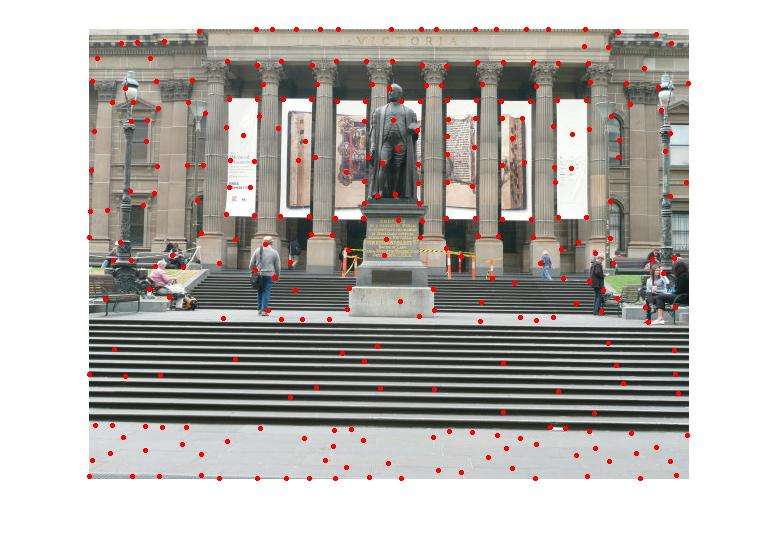
\includegraphics[width=290]{outputimages/ANMS/anms1.jpg}}
% {\caption{This is an example of caption }
% \label{fig1}}
% \end{figure}

% \begin{figure}[t]%
% \FIG{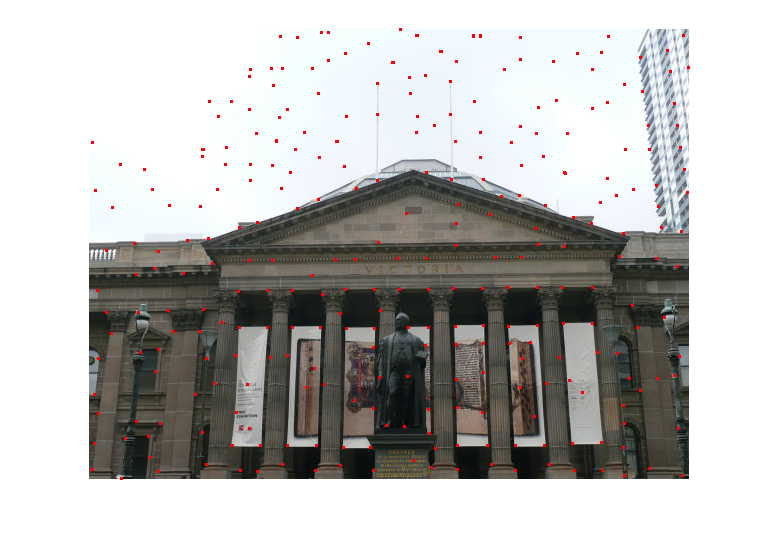
\includegraphics[width=290]{outputimages/ANMS/anms2.png}}
% {\caption{This is an example of caption }
% \label{fig2}}
% \end{figure}

% \begin{figure}[t]%
% \FIG{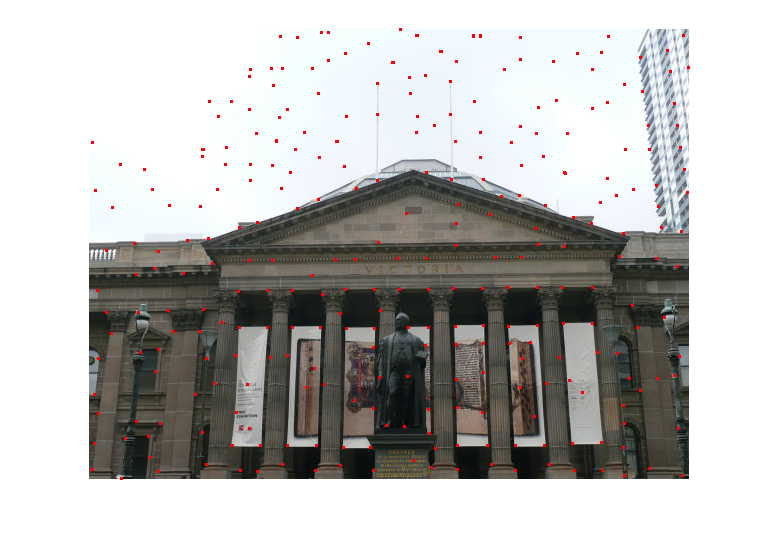
\includegraphics[width=290]{outputimages/ANMS/anms2.png}}
% {\caption{This is an example of caption }
% \label{fig2}}
% \end{figure}
\begin{center}
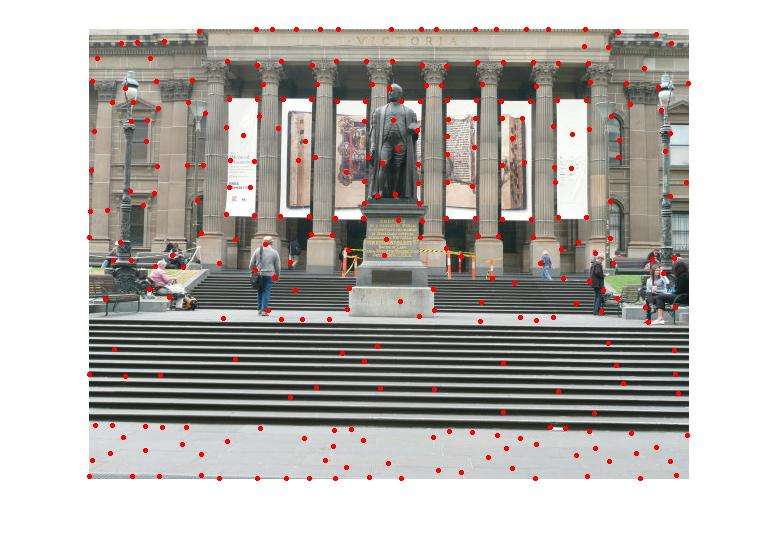
\includegraphics[width=275]{outputimages/ANMS/anms1.jpg}\\
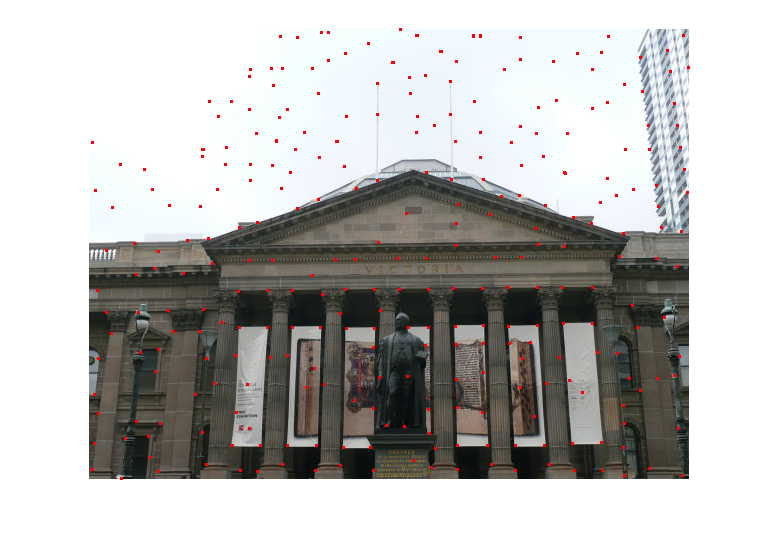
\includegraphics[width=275]{outputimages/ANMS/anms2.png}\\
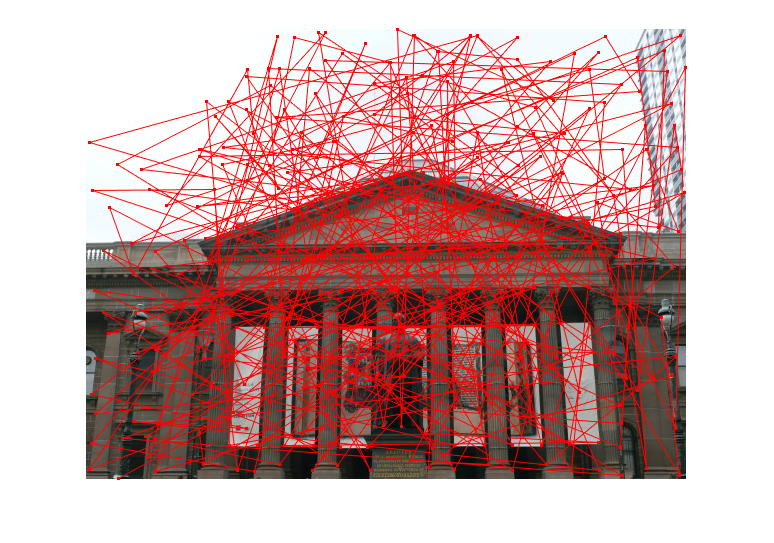
\includegraphics[width=275]{outputimages/ANMS/ANMS4.png}\\
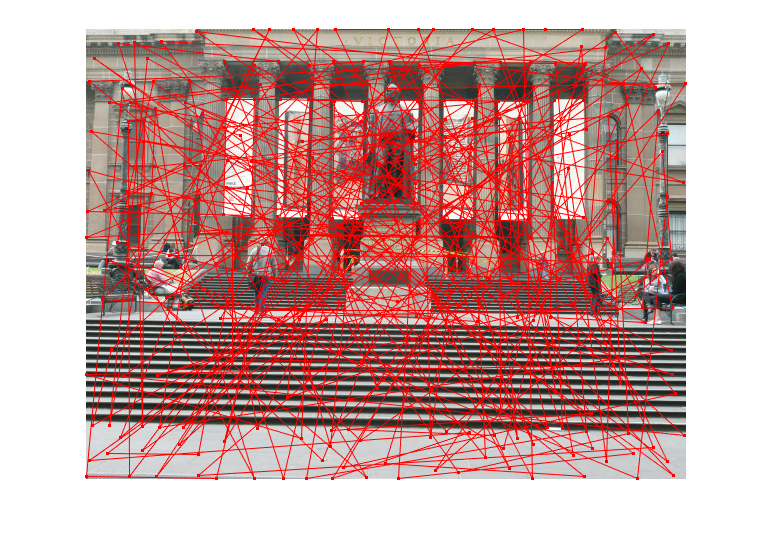
\includegraphics[width=275]{outputimages/ANMS/ANMS5.png}
\end{center}

\section[]{Feature Descriptor}
During the ANMS stage, we discovered feature points. Each feature point must be described by a feature vector, which is equivalent to storing the information at each feature point into a vector. Next, we'll go through one of the most basic feature descriptors.

Take a patch of size 4040 and center it on the key point. At every N-Best point, getFeatureDescriptors() would take a patch around the point ofthe form: I(row-19:row+20, column-19:column+20), blur, reshape and standardize as described.The value is returned as a 64 x N-Best matrix. Apply the gaussian blur to the patch after that. We subsample the blurred output to 8*8 and then shrink the size to 64*1.

\subsection{Shortcoming}
\begin{itemize}
    \item Because the output provides no visible cues, the function is reliant on the accuracy of earlier portions of the project.
    \item The matching discovered enough pairs between the floors (cases of test images - TestSet4) that the whole panorama was influenced in the case of test images - TestSet1.
    \item Before matching, a more robust algorithm may seek the subject first.
\end{itemize}

\section{Feature Matching}


\begin{itemize}
\item
\item 
\item 
\end{itemize}


\section{RANSAC to estimate Robust Homography}
\begin{itemize}
\item
\item 
\item 
\end{itemize}

\section{Blending Images}
To blend images and form a panorama, we need to estimate transformations between images.
Those transformation matrices (H) are estimated using est-(homography()), which takes
coordinates of inliers from RANSAC. We then create a projective2d datatype (tforms) based on each H matrix, then we compute the specific transformation matrix of each image (tforms.T) by applying \\
\begin{equation}
    T(n) = T(n) * T(n-1) * … * T(1)
\end{equation}
The reason for us to do this is that we need to apply several projective2d functions for blending.


\begin{figure}[t]%
\FIG{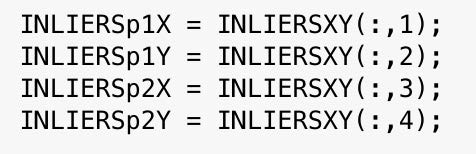
\includegraphics[width=240]{outputimages/blending/p1.jpg}}
{\caption{Figure 1. Example of tforms, projective2d structure}
}
\end{figure}

\begin{figure}[t]%
\FIG{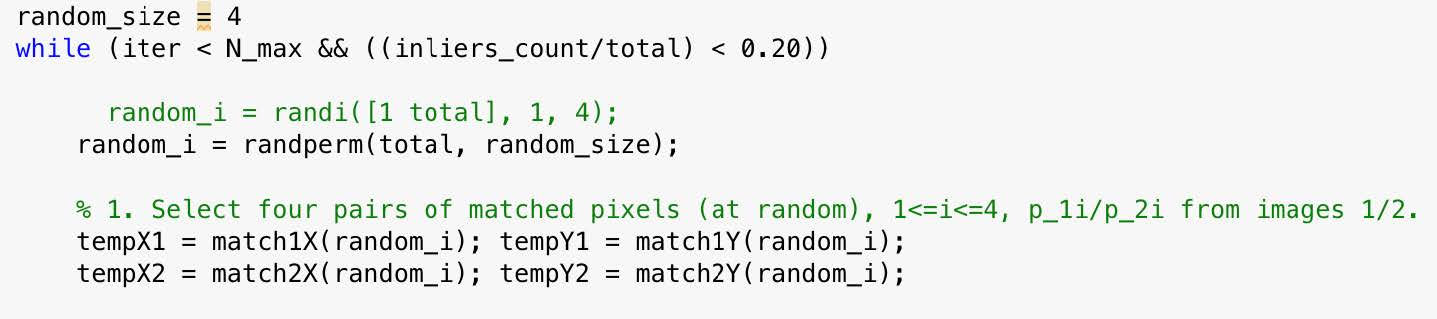
\includegraphics[width=240]{outputimages/blending/p2.jpg}}
{\caption{Figure 2. Reason to apply outputLimits() for transformation}
}
\end{figure}
% 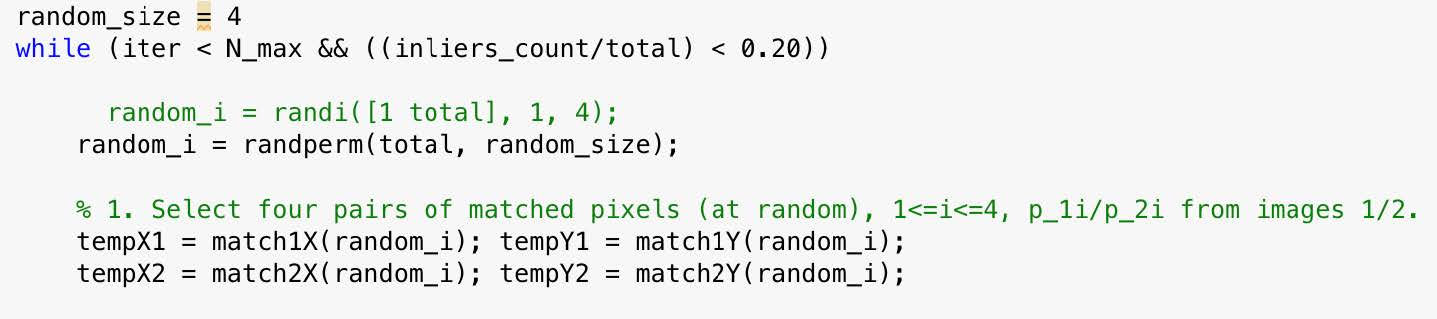
\includegraphics[width=240]{outputimages/blending/p2.jpg}

After we get specific transform matrices, we then calculate coordinate limits for each transform.The reason for us to do this is that images don’t remain in their original shape when they transform. As a result, we need to estimate the limit to make sure we have enough pixel space to hold them after transformations. We uses outputLimits() function from projective2d to achieve this.


To improve the result, we added a step where we recalculate to find a specific picture as the better centerpiece for the panorama. Initially, we estimate all transformations based on the first picture (using the first picture as the center). This action sometimes will make the final panorama looks incorrect if the first picture isn’t a reasonable center (consider if we use an edge picture as the center).
\section{Cylinirical Projection}


\begin{figure}[t]%
\FIG{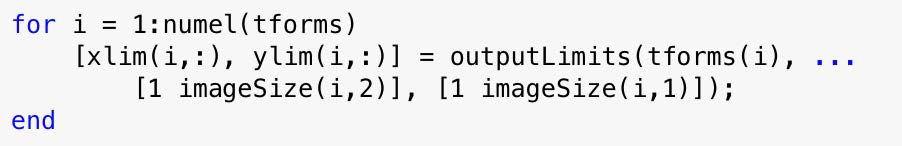
\includegraphics[width=240]{outputimages/blending/p3.jpg}}
{\caption{Figure 3. code portion: outputLimits()}
}
\end{figure}


\begin{figure}[t]%
\FIG{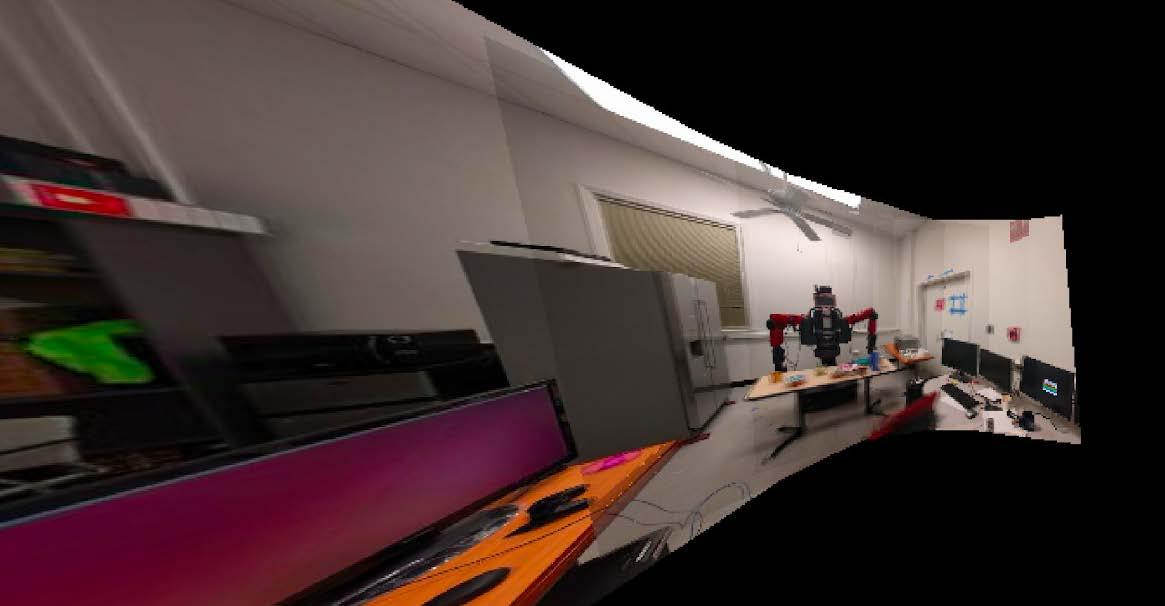
\includegraphics[width=240]{outputimages/blending/p4.jpg}}
{\caption{Figure 4. Example of distorted panorama based on the wrong center}
}
\end{figure}


After we find the new center, we recalculate each picture’s transformation matrix based on it. To do such, we calculate the inverted matrix of the current center’s transformation matrix, and then update other images’ transformation matrices by tforms(i).T = tforms(i).T * Tinv.T. Base on new transformation matrices, we recalculate the limit for each image during transformation. Then, wefind the overall max and min coordinates for all images limit to make sure we have enough space to hold them all for the panorama. Base on the overall max and min, we then initialize the panorama (filled with black pixels).

\begin{figure}[t]%
\FIG{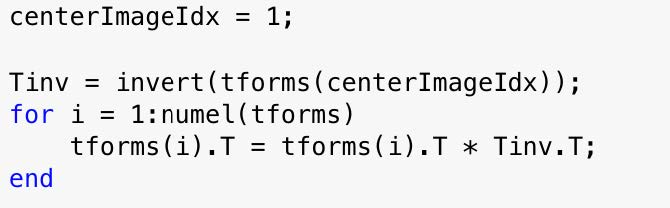
\includegraphics[width=240]{outputimages/blending/p5.jpg}}
{\caption{Figure 5. code portion: Update transformation matrices based on new center Figure}
}
\end{figure}
Finally, we loop through each image, wrap it based on its transformation matrix using imwarp()function, generate a binary mask, then overlay the wrapped image onto the panorama using the step() function. After this stage, we shall have our panorama finished.


% \begin{table}[t]
% \tabcolsep=0pt%
% \TBL{\caption{Tables which are too long to fit,
% should be written using the ``table*'' environment\label{tab2}}}
% {\begin{fntable}
% \begin{tabular*}{\textwidth}{@{\extracolsep{\fill}}lcccccc@{}}\toprule%
%  & \multicolumn{3}{@{}c@{}}{\TCH{Element 1}}& \multicolumn{3}{@{}c@{}}{\TCH{Element 2\smash{\footnotemark[1]}}}
%  \\\cmidrule{2-4}\cmidrule{5-7}%
% \TCH{Project} & \TCH{Energy} & \TCH{$\boldsymbol{\sigma_{\text{calc}}}$} & \TCH{$\boldsymbol{\sigma_{\text{expt}}}$} &
% \TCH{Energy} & \TCH{$\boldsymbol{\sigma_{\text{calc}}}$} & \TCH{$\boldsymbol{\sigma_{\text{expt}}}$} \\\midrule
% \TCH{Stage 3}&990 A &168 &47$\pm$12 &78 A &66 &39$\pm$10\\
% {\TCH{Stage 4}}&500 A &961 &22$\pm$10 &90 A &68 &92$\pm$40\\
% \botrule
% \end{tabular*}%
% \footnotetext[]{{Note:} This is an example of table footnote this is an example of table footnote this is an example of table footnote this is an example of~table footnote this is an example of table footnote}
% \footnotetext[1]{This is an example of table footnote}%
% \end{fntable}}
% \vspace*{7pt}
% \end{table}



\section{Conclusion}

Some Conclusions here.



\begin{Backmatter}
\begin{thebibliography}{}
\bibitem[Ananin and Mironov (2000)]{bib1}
{Ananin, Beth, and Mironov, Antony}. 2000. ``The moduli space of $2$-dimensional algebras'', \textit{Comm. Algebra} {28}(9),  {4481}--{4488}.

\bibitem[Bai and Meng (2001)]{bib2}
{Bai, Clifton, and Meng, Dyck}. 2001. ``The classification of Novikov algebras in low dimension'',  \textit{J. Phys. A: Math. Gen.} {34}, {1581}--{1594}.

\bibitem[Ca\~{n}ete and Khudoyberdiyev (2013)]{bib3}
{Ca\~{n}ete, Enderson, and Khudoyberdiyev, Angus}. 2013. ``The classification of $4$-dimensional Leibniz algebras'',  \textit{Linear Algebra and its Applications}  {439}(1), {273}--{288}.

\bibitem[Goze and Remm (2011)]{bib4}
{Goze, Michael, and Remm, Edward}. 2011.  ``$2$-dimensional algebras'',  \textit{Afr. J. Math. Phys.} {10}(1),  {81}--{91}.

\bibitem[Petersson (2000)]{bib5}
{Petersson, Hentry}. 2000. ``The classification of two-dimensional nonassociative algebras'',  \textit{Results Math} {37}, no. 1-2,  {120}--{154}.

\end{thebibliography}

\end{Backmatter}
\end{document}
